\chapter{Arhitektura i dizajn sustava}
		
	Za arhitekturu sustava odabrali smo klasičan klijent-server pristup. \\
	
	\textbf{Klijent}\\
	Strana klijenta je web stranica izgrađena u programskom jeziku JavaScript uz pomoć biblioteke React. Odabrali smo ovu tehnologiju jer je React danas najkorištenija biblioteka za razvoj web stranica i kao takva nudi najbolji ekosustav funkcionalnosti i podrške. Korišteno razvojno okruženje je VScode. Zadatak klijenta je slanje zahtjeva prema serveru koji ih zatim obrađuje. Svi zahtjevi se šalju pomoću HTTP POST metode i šalju se u JSON formatu prema serveru.\\
	
	\textbf{Server}\\
	Za server stranu odabrali smo programski jezik Javu i razvojno okruženje \textit{Spring Boot}. \textit{Spring Boot} smo odabrali jer je standardno razvojno okruženje za jezik Javu, a Javu smo odabrali kako bismo na prirodan način mogli sustav implementirati koristeći objektno orijentiranu paradigmu. Za razvoj serverskog koda korišten je alata Intellij IDEA. \textit{Spring Boot} nam također nudi neke dodate pogodnosti kao što je proširenje \textit{Spring Security} koje znatno olakšava proces implementacije sigurnog i točnog procesa prijave i registracije korisnika. Server prima zahtjeve od klijenta u JSON formatu i pretvara te zahtjeve u Java objekte nad kojima izvršava daljnje operacije. Kada server obradi zahtjev šalje natrag HTTP odgovor s odgovarajućim statusnim kodom kako bi klijent znao je li operacija uspjela ili nije.
		

		

				
		\section{Baza podataka}
			
		 Kao sustav za upravljanje bazama podataka odabrali smo PostgreSQL. Implementacija naše PostgreSQL baze podataka obuhvaća nekoliko ključnih elemenata, uključujući organizaciju podataka u tablicama i uspostavljanje veza između tablica radi složenih upita. Baza podatka sastoji se od slijedećih entiteta: 
		
		\begin{packed_item}
			\item KLINIKA
			\item SMJEŠTAJ
			\item PRIJEVOZNIK
			\item VOZILO
			\item KORISNIK
			\item PUTOVANJE
		\end{packed_item}
		
			\subsection{Opis tablica}
			
				\textbf{KLINIKA}\hspace{0.5cm}Entitet KLINIKA sadrži informacije o ID-u klinike, nazivu i adresi. Prema tome, entitet KLINIKA posjeduje sljedeće atribute: IDKlinika, naziv i adresa. Entitet KLINIKA je u vezi \textit{One-to-Many} s entitetom SMJESTAJ preko atributa IDKlinika i u vezi \textit{One-to-Many} s enitetom PUTOVANJE preko atributa IDKlinika. Također je u \textit{One-to-Many} vezi s enitetom PUTOVANJE preko atributa adresa.
				
				\begin{longtblr}[
					label=none,
					entry=none
					]{
						width = \textwidth,
						colspec={|X[6,l]|X[6, l]|X[20, l]|}, 
						rowhead = 1,
					} %definicija širine tablice, širine stupaca, poravnanje i broja redaka naslova tablice
					\hline \SetCell[c=3]{c}{\textbf{KLINIKA}}	 \\ \hline[3pt]
					\SetCell{LightGreen}IDKlinika & INT	& Identifikacijski ključ klinike	\\ \hline
					naziv	& VARCHAR & Naziv klinike\\ \hline 
					adresa & VARCHAR & Adresa klinike\\ \hline 
				\end{longtblr}
				
				\textbf{SMJESTAJ}\hspace{0.5cm}Entitet SMJESTAJ sadrži podatke o ID-u smještaja, tipu stana, kategoriji opremljenosti, adresi kao i vremenskom periodu dostupnosti za korištenje. Sukladno tome, entitet SMJESTAJ posjeduje sljedeće atribute: IDSmjestaj, tip, kategorija, adresa i dostupnost. Entiet SMJESTAJ je u vezi  \textit{Many-to-One} s entitetom KLINIKA preko atributa IDKlinika i u vezi  \textit{One-to-Many} s enitetom PUTOVANJE preko atributa IDPutovanje. Također je u \textit{One-to-Many} vezi s enitetom PUTOVANJE preko atributa adresa.
				
				\begin{longtblr}[
					label=none,
					entry=none
					]{
						width = \textwidth,
						colspec={|X[6,l]|X[6, l]|X[20, l]|}, 
						rowhead = 1,
					} %definicija širine tablice, širine stupaca, poravnanje i broja redaka naslova tablice
					\hline \SetCell[c=3]{c}{\textbf{SMJESTAJ}}	 \\ \hline[3pt]
					\SetCell{LightGreen}IDSmjestaj & INT	&  Identifikacijski ključ smještaja	\\ \hline
					tip	& VARCHAR &  Tip stana\\ \hline 
					kategorija & VARCHAR & Kategorija opremljenosti  \\ \hline 
					adresa & VARCHAR	&  Adresa smještaja\\ \hline 
					dostupnost & INTERVAL	&  Vremenski period dostupnosti za korištenje\\ \hline 
					\SetCell{LightBlue} IDKlinika & INT	&  Identifikacijski ključ klinike  	\\ \hline 
				\end{longtblr}
				
				\textbf{PRIJEVOZNIK}\hspace{0.5cm}Entitet PRIJEVOZNIK sadrži informacije o ID-u prijevoznika, kontaktnim podacima i o radnom vremenu u kojem je prijevoznik raspoloživ. Prema tome, entitet PRIJEVOZNIK posjeduje sljedeće atribute: IDPrijevoznik, kontakt i radnoVrijeme. Entitet PRIJEVOZNIK je u vezi \textit{One-to-Many} s entitetom VOZILO preko atributa IDPrijevoznik i u vezi \textit{One-to-Many} s enitetom PUTOVANJE preko atributa IDPrijevoznik.
				
				
				\begin{longtblr}[
					label=none,
					entry=none
					]{
						width = \textwidth,
						colspec={|X[6,l]|X[6, l]|X[20, l]|}, 
						rowhead = 1,
					} %definicija širine tablice, širine stupaca, poravnanje i broja redaka naslova tablice
					\hline \SetCell[c=3]{c}{\textbf{PRIJEVOZNIK}}	 \\ \hline[3pt]
					\SetCell{LightGreen}IDPrijevoznik & INT	& Identifikacijski ključ prijevoznika	\\ \hline
					kontakt	& VARCHAR &  Kontaktni podatci prijevoznika	\\ \hline 
					radnoVrijeme & TIME & Radno vrijeme u kojem su prijevoznici raspoloživi  \\ \hline 
				\end{longtblr}
				
				\textbf{VOZILO}\hspace{0.5cm}Entitet VOZILO sadrži informacije o ID-u vozila, vrsti i kapacitetu prijevoznog sredstva. Prema tome, entitet VOZILO posjeduje sljedeće atribute: IDVozilo, vrsta i kapacitet. Entitet VOZILO je u vezi \textit{Many-to-One} s entitetom PRIJEVOZNIK preko atributa IDPrijevoznik.
				
				\begin{longtblr}[
					label=none,
					entry=none
					]{
						width = \textwidth,
						colspec={|X[6,l]|X[6, l]|X[20, l]|}, 
						rowhead = 1,
					} %definicija širine tablice, širine stupaca, poravnanje i broja redaka naslova tablice
					\hline \SetCell[c=3]{c}{\textbf{VOZILO}}	 \\ \hline[3pt]
					\SetCell{LightGreen}IDVozilo & INT	&  Identifikacijski ključ vozila	\\ \hline
					vrsta	& VARCHAR & Vrsta vozila\\ \hline 
					kapacitet & VARCHAR & Kapacitet vozila\\ \hline 
					\SetCell{LightBlue} IDPrijevoznik & INT	& Identifikacijski ključ prijevoznika   	\\ \hline 
				\end{longtblr}
				
				\textbf{KORISNIK}\hspace{0.5cm}Entitet KORISNIK sadrži informacije o ID-u korisnika, imenu, prezimenu, kontaktnim podacima i preferencijama vezanim uz veličinu i kvalitetu smještaja. Prema tome, entitet KORISNIK posjeduje sljedeće atribute: IDKorisnik, ime, prezime, kontakt i preferencije. Entitet KORISNIK je u vezi \textit{One-to-Many} s enitetom PUTOVANJE preko atributa IDKorisnik.
				
				\begin{longtblr}[
					label=none,
					entry=none
					]{
						width = \textwidth,
						colspec={|X[6,l]|X[6, l]|X[20, l]|}, 
						rowhead = 1,
					} %definicija širine tablice, širine stupaca, poravnanje i broja redaka naslova tablice
					\hline \SetCell[c=3]{c}{\textbf{KORISNIK}}	 \\ \hline[3pt]
					\SetCell{LightGreen}IDKorisnik & INT	&  Identifikacijski ključ korisnika	\\ \hline
					ime	& VARCHAR & Ime korisnika	\\ \hline 
					prezime & VARCHAR & Prezime korisnika \\ \hline
					kontakt & VARCHAR & Kontakt korisnika \\ \hline 
					preferencije & VARCHAR	& Preferencije vezane uz veličinu i kvalitetu smještaja\\ \hline 
				\end{longtblr}
				
				\textbf{PUTOVANJE}\hspace{0.5cm}Entitet PUTOVANJE sadrži informacije o ID-u putovanja, vremenu i smjeru putovanja. Prema tome, entitet PUTOVANJE posjeduje sljedeće atribute: IDPutovanje, vrijeme i smjer. Entitet PUTOVANJE j u vezi \textit{Many-to-One} s enitetom KLINIKA preko atributa IDKorisnik, u vezi \textit{Many-to-One} s enitetom SMJESTAJ preko atributa IDSmjestaj, u vezi \textit{Many-to-One} s enitetom KORISNIK preko atributa IDKorisnik, u vezi \textit{Many-to-One} s enitetom PRIJEVOZNIK preko atributa IDPrijevoznik. Atributi adresa1 i adresa2 su atributi iz kojih saznajemo adresu polaska ili dolaska u ovisnosti o smjeru koji može biti 1 ili 0. Entitet PUTOVANJE u vezi je \textit{Many-to-One} s enitetom KLINIKA preko atributa adresa1, u vezi \textit{Many-to-One} s enitetom SMJESTAJ preko atributa adresa2.
				
				\begin{longtblr}[
				label=none,
				entry=none
					]{
						width = \textwidth,
						colspec={|X[6,l]|X[6, l]|X[20, l]|}, 
						rowhead = 1,
					} %definicija širine tablice, širine stupaca, poravnanje i broja redaka naslova tablice
					\hline \SetCell[c=3]{c}{\textbf{PUTOVANJE}}	 \\ \hline[3pt]
					\SetCell{LightGreen}IDPutovanje & INT	&  Identifikacijski ključ putovanja	\\ \hline
					vrijeme	& TIME &  Vrijeme putovanja	\\ \hline 
					smjer & INT &  Smjer u kojem se putovanje izvodi \\ \hline 
					\SetCell{LightBlue} adresa1 & VARCHAR	&  Adresa klinike\\ \hline
					\SetCell{LightBlue} adresa2 & VARCHAR	& Adresa smještaja\\ \hline 
					\SetCell{LightBlue} IDKorisnik & INT	&  Identifikacijski ključ korisnika	\\ \hline 
					\SetCell{LightBlue} IDKlinika & INT	& Identifikacijski ključ klinike	\\ \hline
					\SetCell{LightBlue} IDPrijevoznik & INT	& Identifikacijski ključ prijevoznika	\\ \hline
					\SetCell{LightBlue} IDSmjestaj & INT	& Identifikacijski ključ smještaja	\\ \hline
				\end{longtblr}
				
			\eject
			
			\subsection{Dijagram baze podataka}
					
				\begin{figure}[htbp]
					\centering
					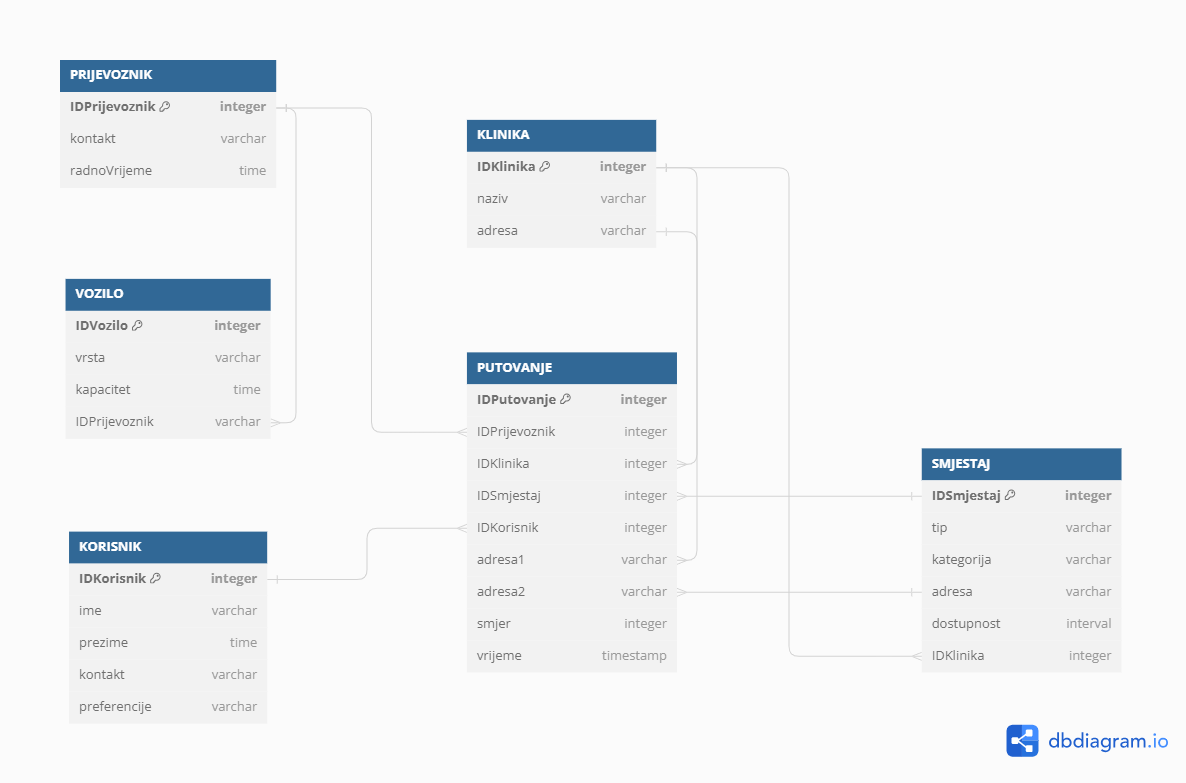
\includegraphics[width=0.9\textwidth]{slike/bazaPodataka.png}
					\caption{Relacijska shema baze podataka}
					\label{fig:bazaPodataka}
				\end{figure}
				
			
			\eject
			
			
		\section{Dijagram razreda}
		
			
			Slika~\ref{fig:controllers} prikazuje razred \textit{AuthController} koji služi prihvaćanju HTTP zahtjeva od strane klijenta i to specifično za URL \textit{/auth/**}. Metode \textit{login()} i \textit{register()} služe kao URL-ovi \textit{/auth/login} i \textit{/auth/register} na koje se šalju JSON objekti za prijavu administratora i registraciju novog administratora. Prikazan su i razredi: \textit{PrijevozController}, \textit{KorisnikController},  \textit{PrijevozController} i \textit{SmjestajniController}. Metode unutar tih razreda izvršavaju manipulacije nad modelima i vraćaju tražene informacije koje su predstavljene modelima, obično u obliku listi podataka. 
			
			Modeli su prikazani slikom~\ref{fig:models}. Razredi modela preslikavaju strukturu baze podataka u okviru aplikacije. Razredi odgovaraju entitetima iz baze podataka.
			
			\begin{figure}[htbp]
				\centering
				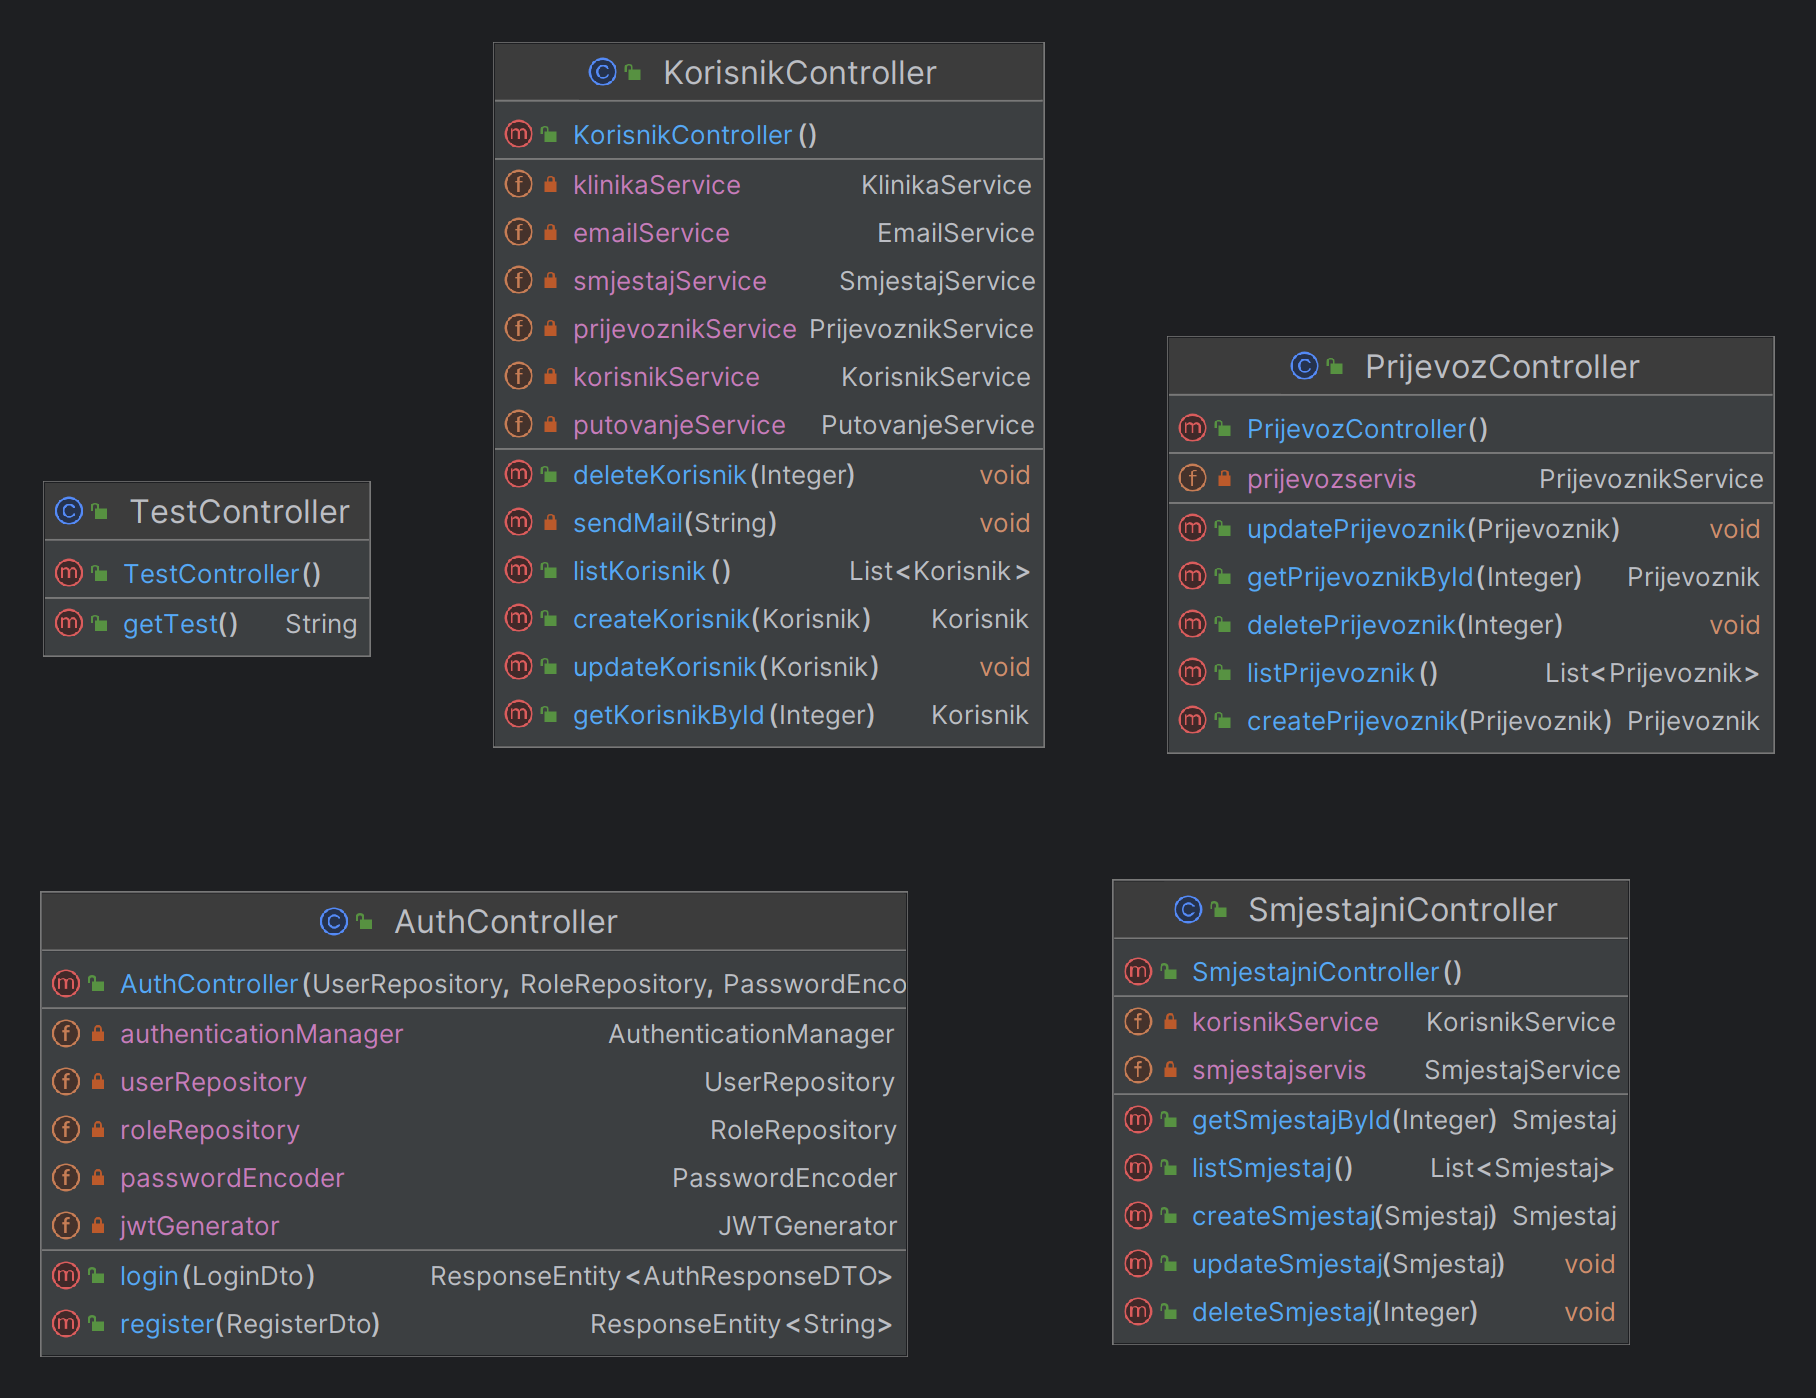
\includegraphics[width=0.9\textwidth]{slike/controllers}
				\caption{\textit{Controllers}}
				\label{fig:controllers}
			\end{figure}
			
			\begin{figure}[htbp]
				\centering
				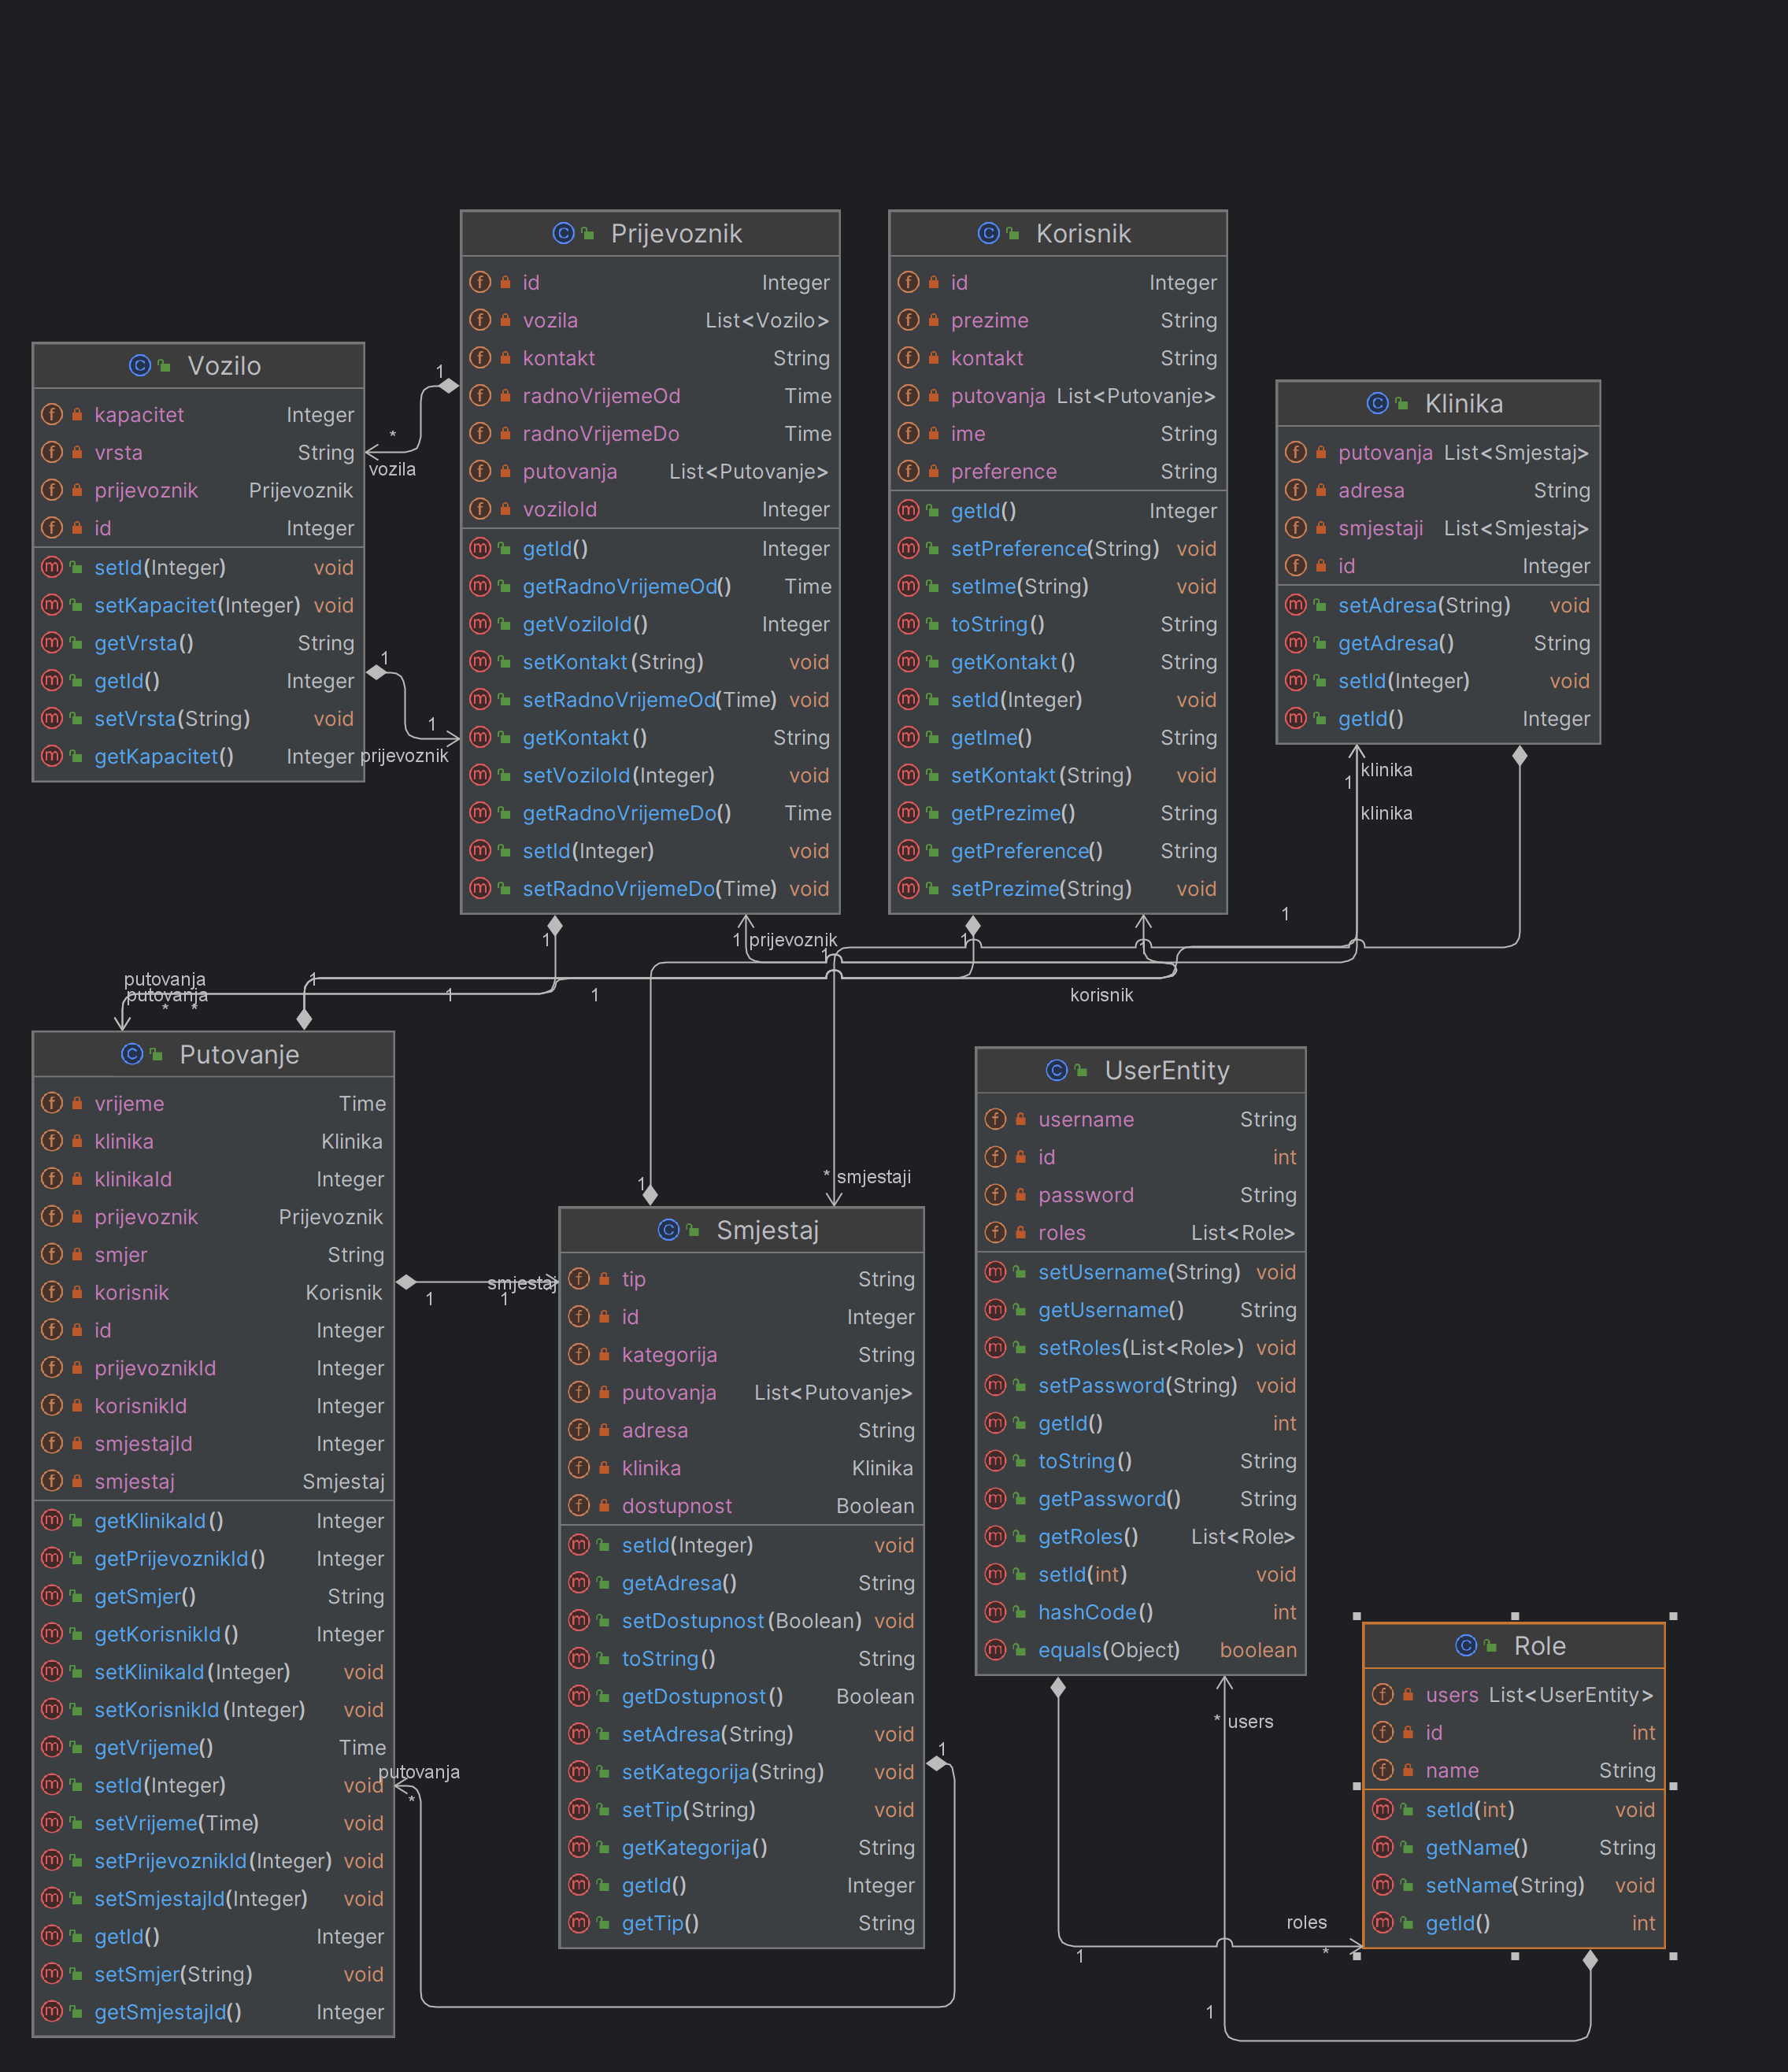
\includegraphics[width=0.9\textwidth]{slike/models}
				\caption{UML dijagram paketa \textit{Models}}
				\label{fig:models}
			\end{figure}
			
			\eject
			
			Slika~\ref{fig:dto} prikazuje paket DTO koji služi za pretvaranje JSON objekata koji stižu na određenu rutu i Java objekt i za pretvaranje Java objekata u JSON odgovore koje klijent razumije.
			Između razreda Controllers i DTO ne postoje veze na dijagramima.
			
			\begin{figure}[htbp]
				\centering
				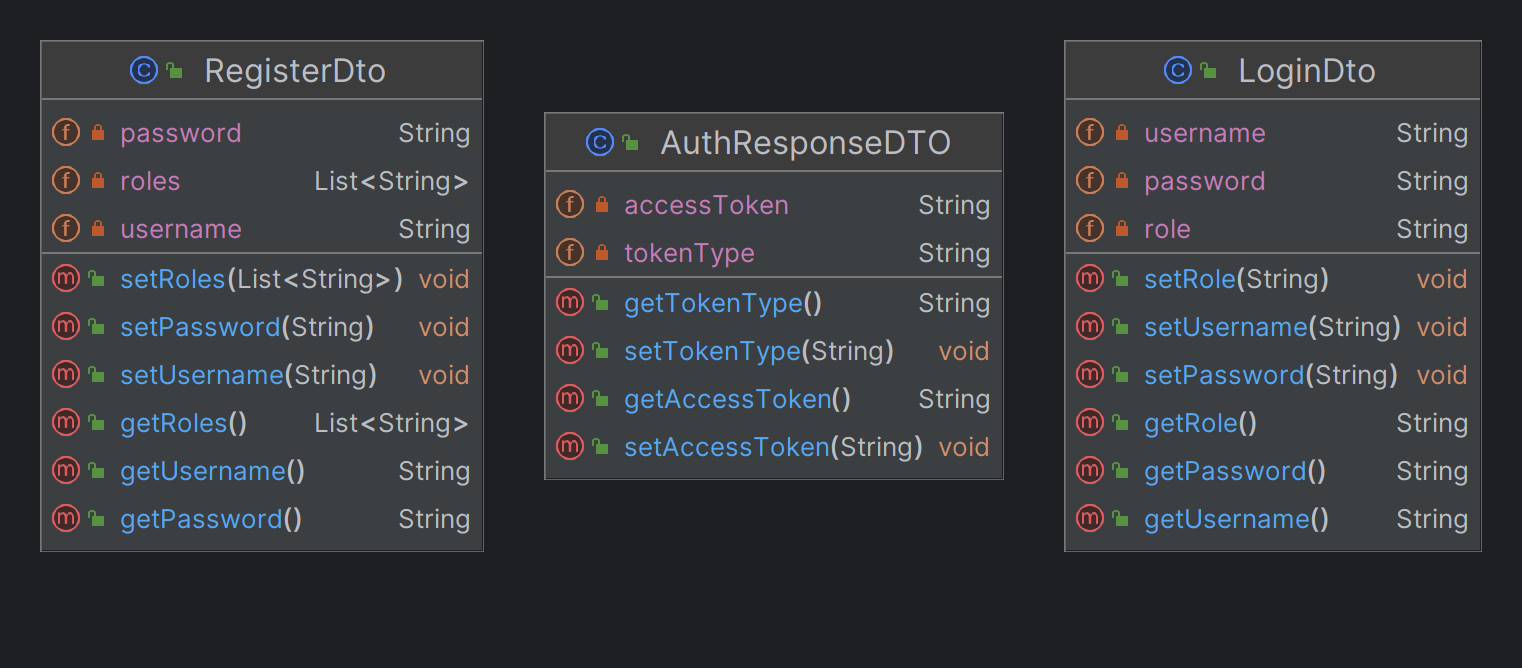
\includegraphics[width=0.9\textwidth]{slike/dto}
				\caption{\textit{DTO}}
				\label{fig:dto}
			\end{figure}
			
			
			Slika~\ref{fig:security} prikazuje paket \textit{Security} koji je zadužen za obradu svakog zahtjeva koji stiže na server i prosuditi ima li trenutni korisnik pravo pristupa. Glavna klasa za to je klasa \textit{SecurityConfig} koja preko metode \textit{filterChain()} primjenjuje filtre na svaki zahtjev da odredi pravo pristupa. Također klasa \textit{SecurityConfig} pomoću klasa \textit{JWTGenerator, JWTAuthenticationFilter i JwtAuthEntryPoint} za svaku uspješnu prijavu generira JWT token koji se zatim u svim zahtjevima tog korisnika koristi za autentifikaciju tog korisnika.
			
			\begin{figure}[htbp]
				\centering
				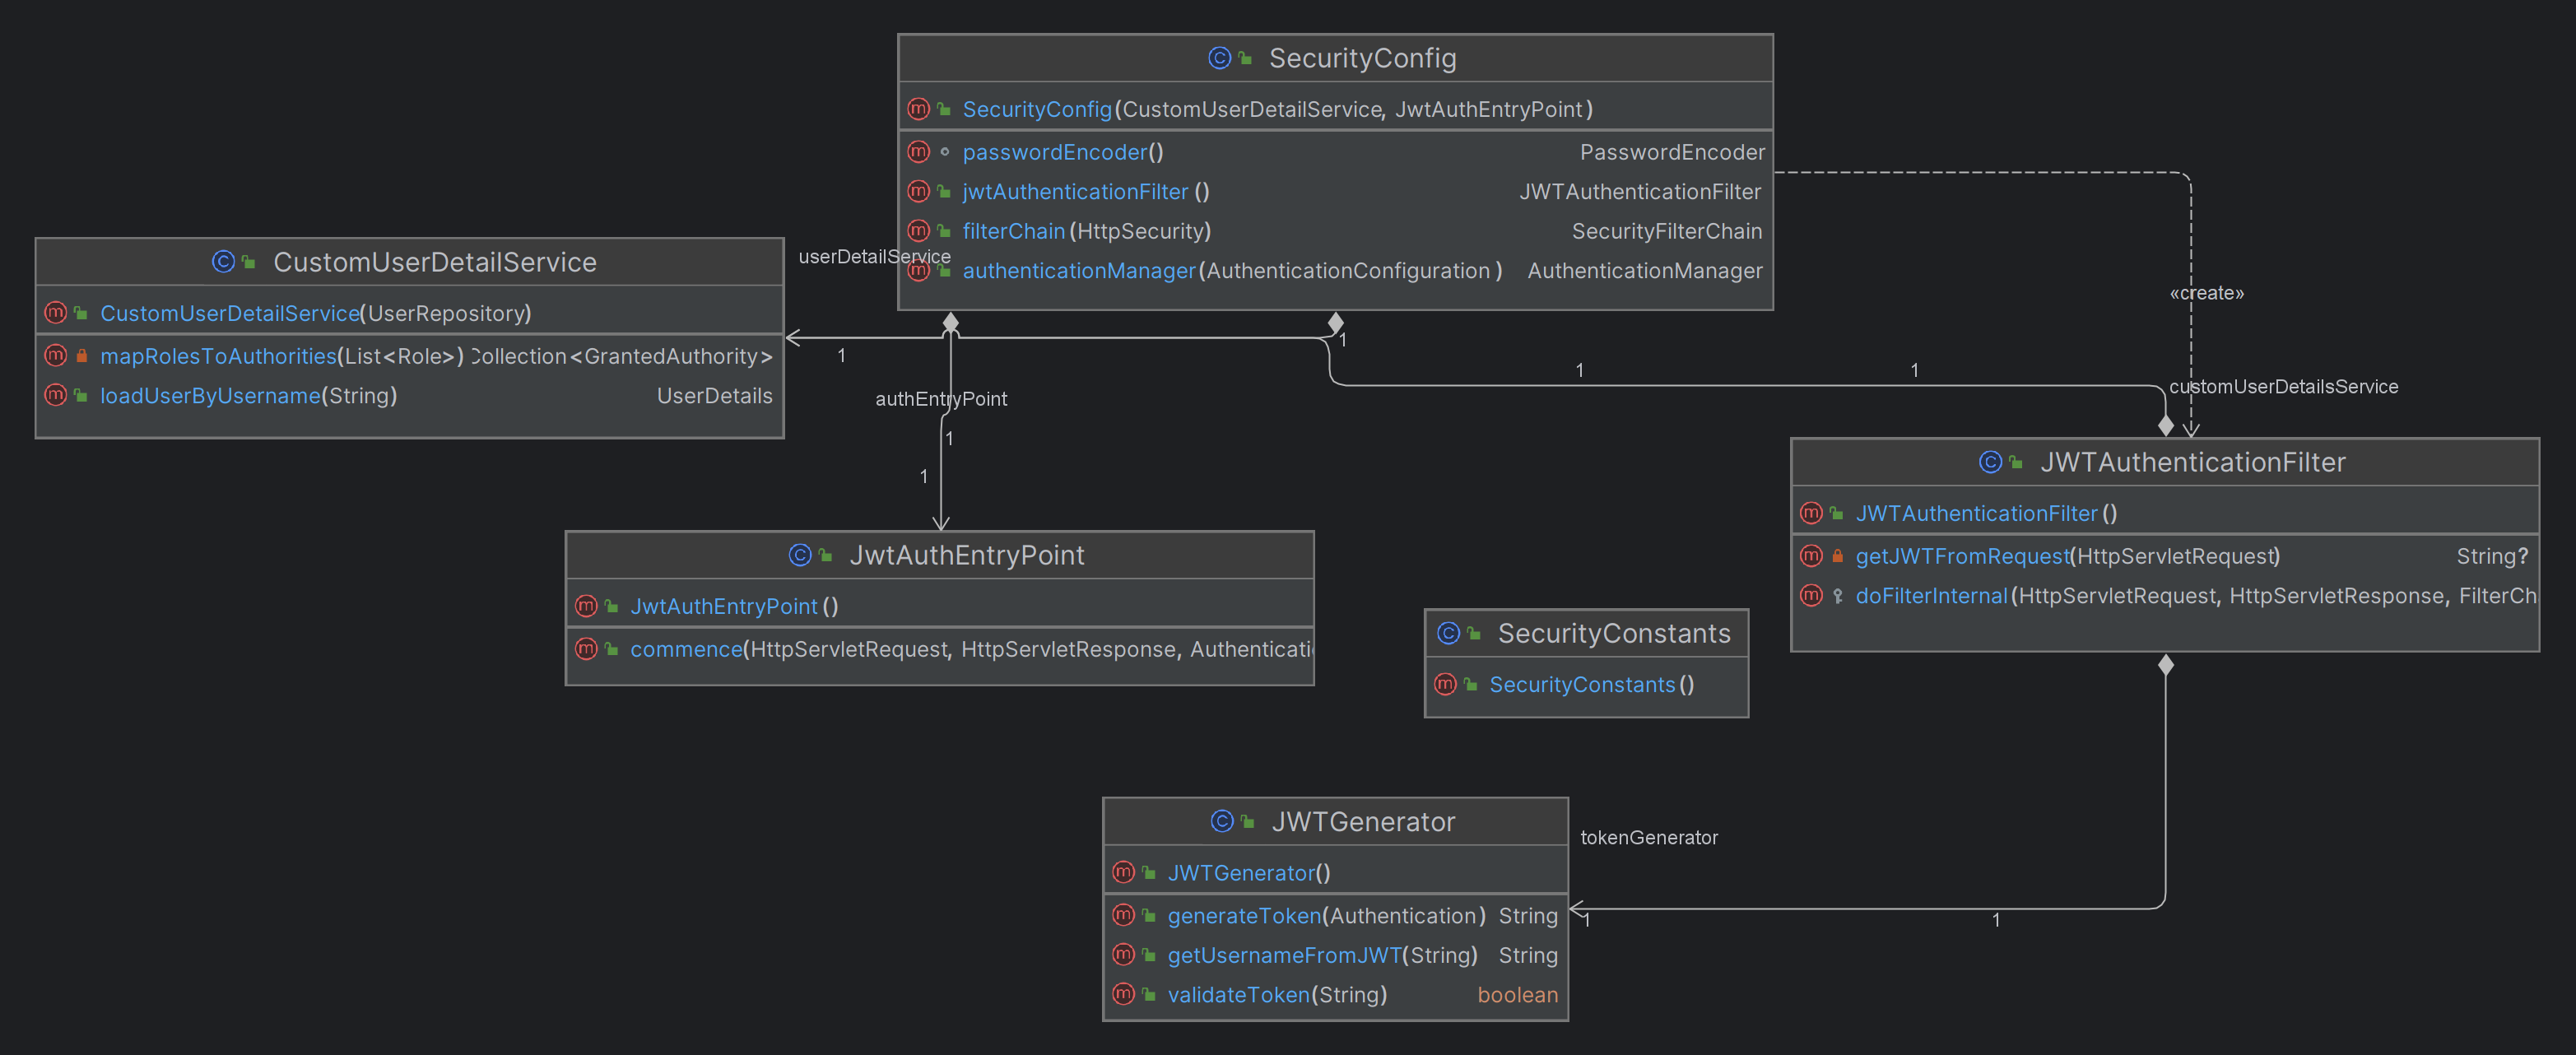
\includegraphics[width=0.9\textwidth]{slike/security}
				\caption{UML dijagram paketa \textit{Security}}
				\label{fig:security}
			\end{figure}
			
			\eject
			
			Slika~\ref{fig:security} prikazuje paket \textit{DAO}. Paket \textit{DAO} ima odgovornost za pristup podacima u sustavu i interakciju s bazom podataka. Implementacije razreda unutar ovog paketa, kao što su \textit{PutovanjeDaoImpl}, \textit{SmjestajDaoImpl}, \textit{KlinikaDaoImpl}, \textit{VoziloDaoImpl}, \textit{PrijevoznikDaoImpl} i \textit{KorisnikDaoImpl}, služe za implementaciju funkcija koje upravljaju bazom podataka. Ovi razredi omogućavaju izvođenje operacija čitanja, pisanja, ažuriranja i brisanja podataka u odgovarajućim entitetima sustava.
			
			\begin{figure}[htbp]
				\centering
				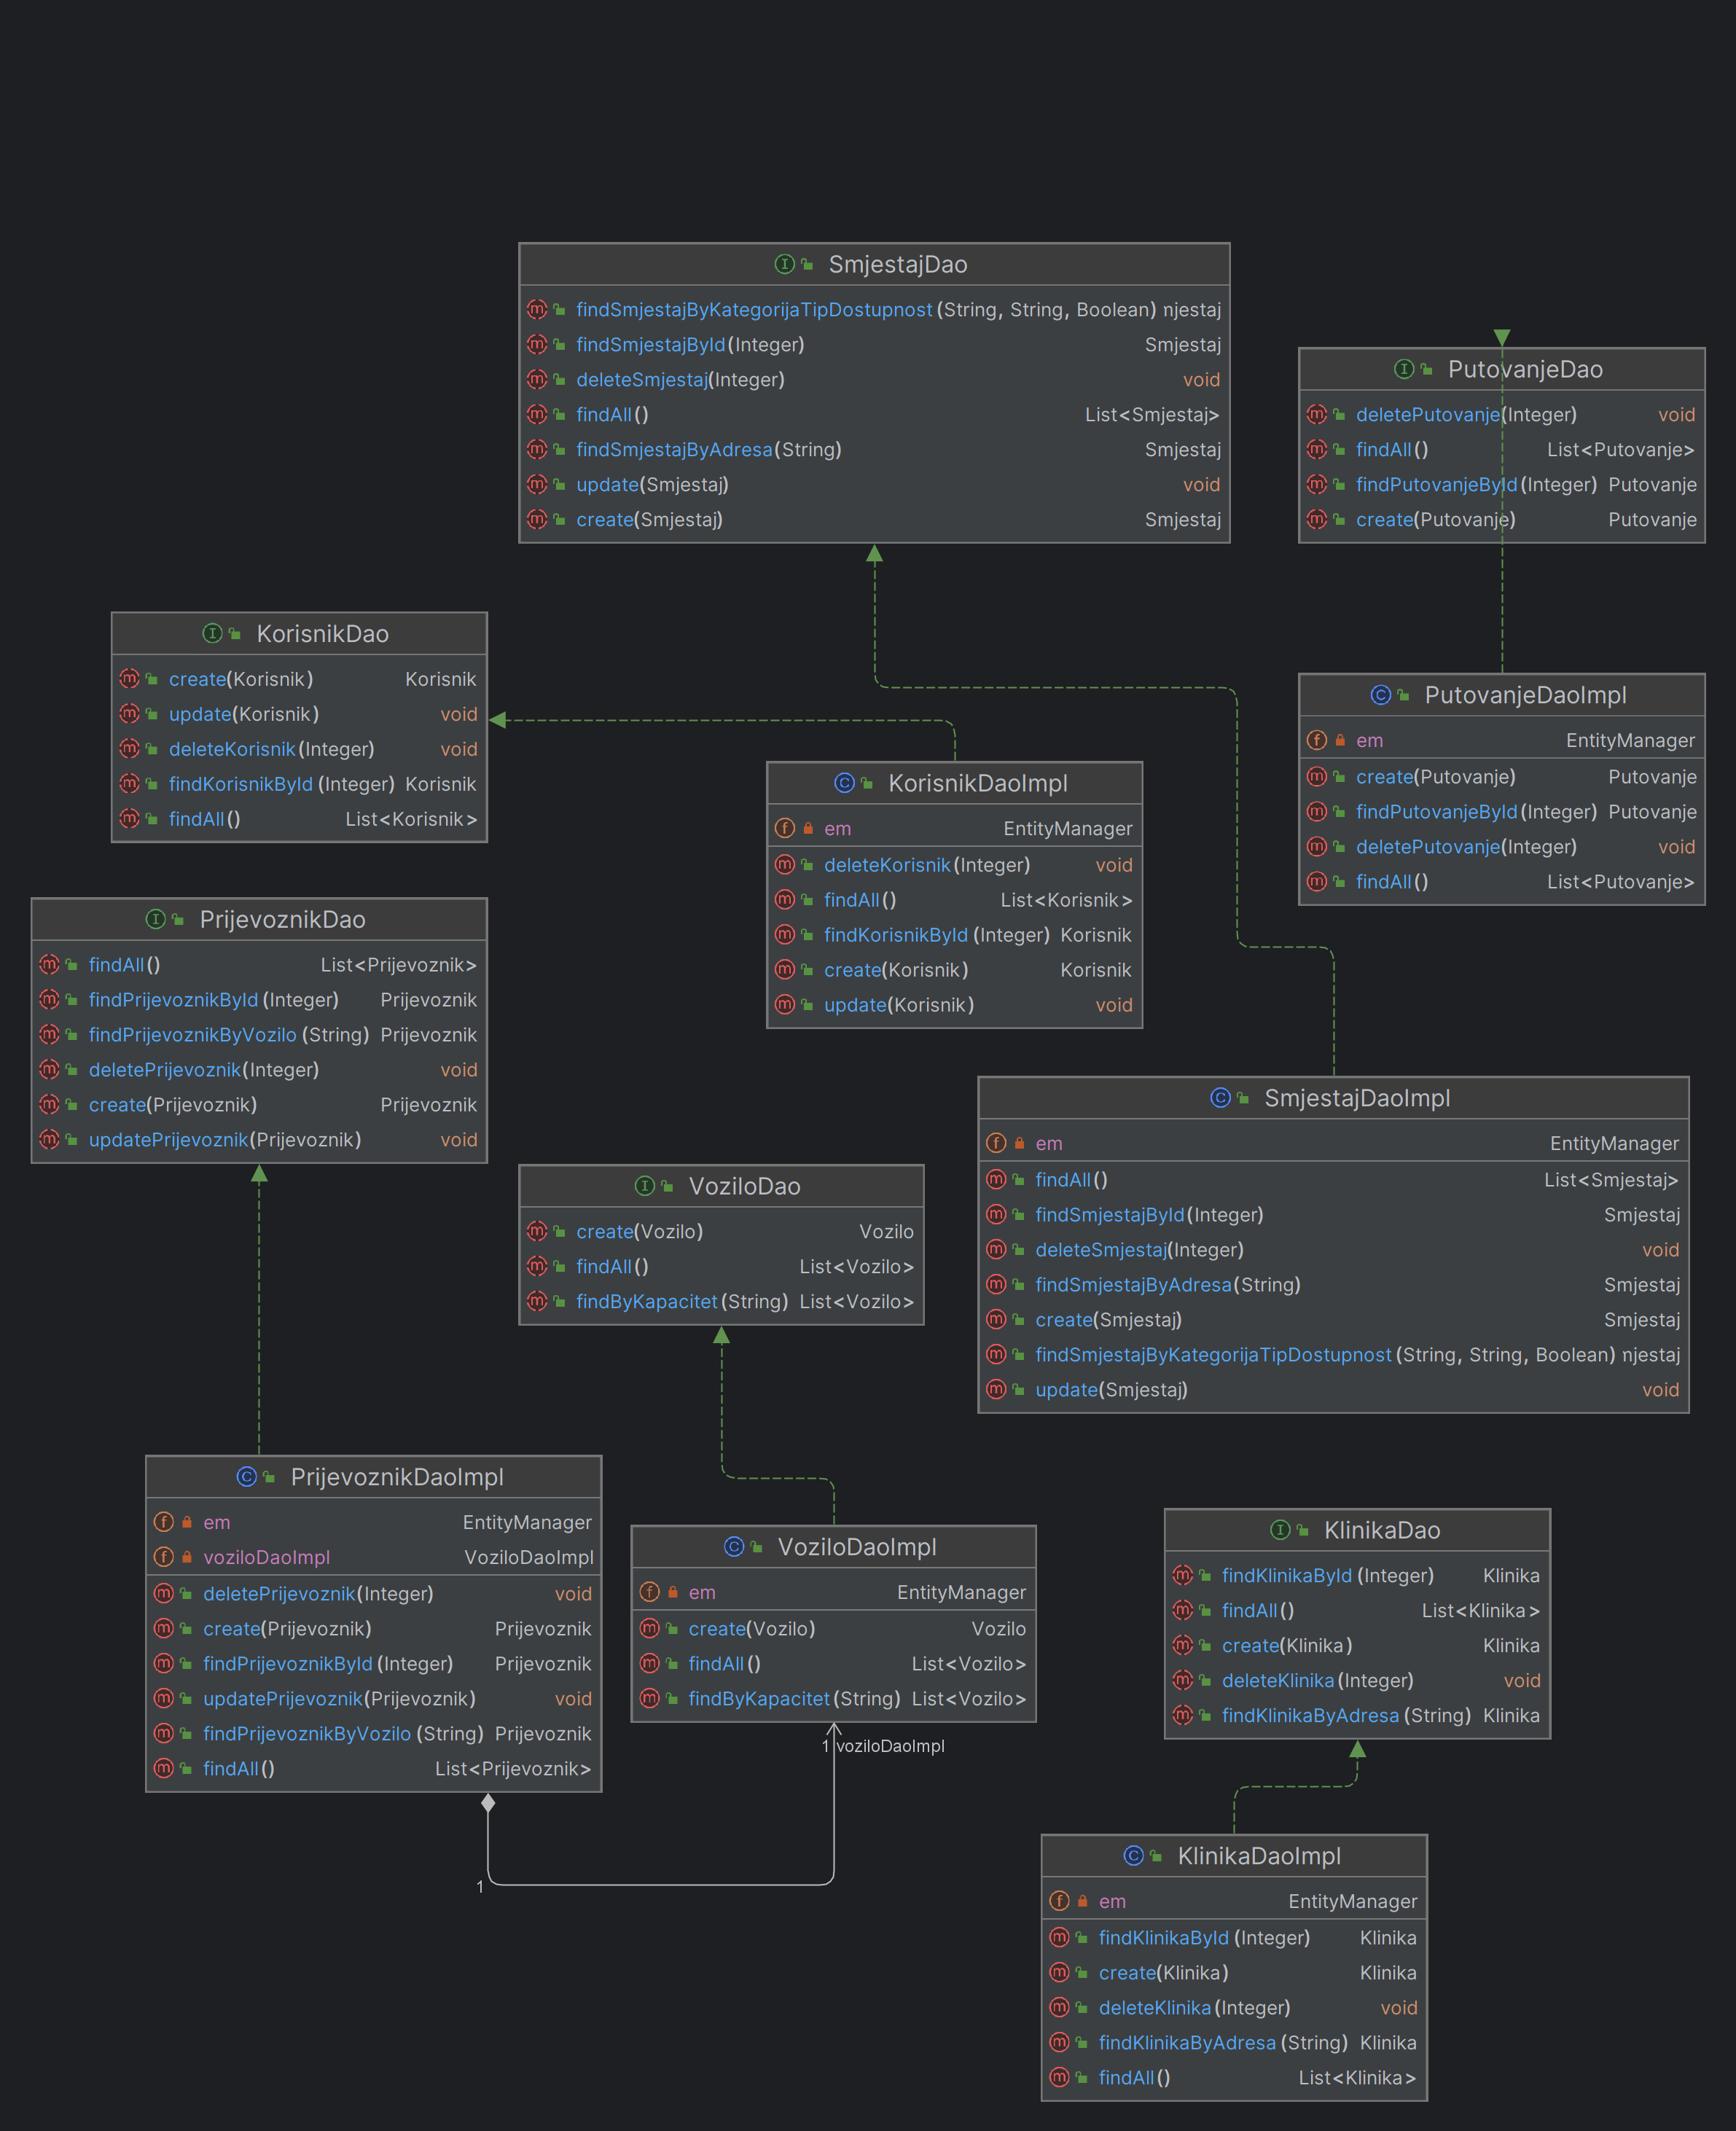
\includegraphics[width=0.9\textwidth]{slike/dao}
				\caption{UML dijagram paketa \textit{DAO}}
				\label{fig:dao}
			\end{figure}
			
			\eject
		
		\section{Dijagram stanja}
			
			
			Na slici~\ref{fig:dijagramStanja} prikazan je dijagram stanja. Dijagram stanja prikazuje u kojem se stanju korisnik aplikacije može nalaziti. Početno stanje je prijava. Korisnik se može prijaviti kao jedan od administratora: Korisnički administrator, Smještajni administrator ili Prijevozni administrator. Ovisno o tome koji administrator se prijavi, odlazi na odgovarajuću početnu stranicu (homepage) gdje se nalaze opcije za korištenje ovisno o ulozi. Svi administratori mogu se vratiti na prijavu tako što se prethodno odjave, klikom "Odjava".
			
			Ako je prijavljeni administrator smještajni administrator, ima opciju dodavanja novih administratora odabirom opcije "Dodaj admina". Također, ima mogućnost pregleda smještaja i ažuriranja istog pomoću opcije "Ažuriraj". Već postojeći smještaj administrator može obrisati opcijom "Obriši". Novi smještaj dodaje opcijom "Dodaj".
			
			Ako je prijavljeni administrator prijevozni administrator, ima opciju pregleda već postojećih prijevoznika te ažuriranja istih opcijom "Ažuriraj". Također, prijevozni administrator može dodavati nove prijevoznike opcijom "Dodaj" i brisati već postojeće opcijom "Obriši".
			
			Ako je prijavljeni administrator korisnički administrator, ima opciju dodavanja novog korisnika (klijenta) opcijom "Dodaj". Također, odabirom korisnika mogu se pregledavati njegovi podaci te odabirom opcije "Ažuriraj" ažurirati. Korisnike se može brisati opcijom "Obriši".
			
			\begin{figure}[htbp]
				\centering
				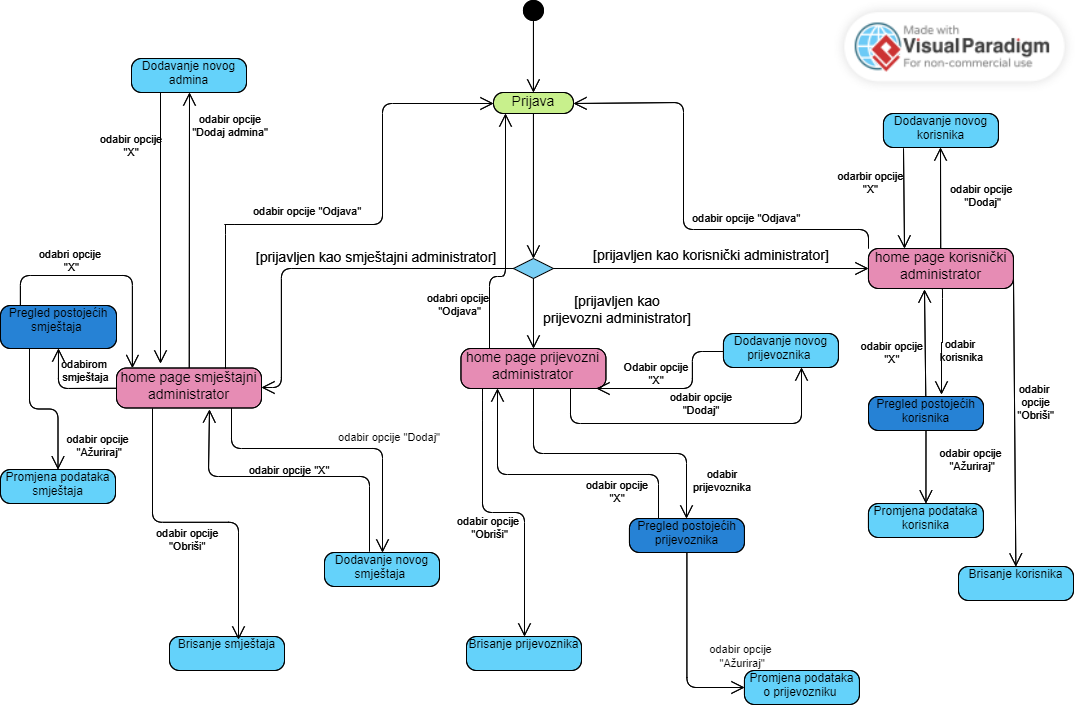
\includegraphics[width=0.9\textwidth]{dijagrami/dijagramStanja.png}
				\caption{Dijagram stanja}
				\label{fig:dijagramStanja}
			\end{figure}
			
			
			\eject 
			\clearpage
			
		\section{Dijagram aktivnosti}
		
				Na slici~\ref{fig:dijaramAktivnosti} prikazan je dijagram aktivnosti. Dijagram aktivnosti ilustrira detalje procesa kreiranja rezervacije za korisnika putem web-aplikacije. Korisnički administrator započinje postupak unosom ispravnih podataka za prijavu u web-aplikaciju. Ukoliko se uneseni podaci pokažu neispravnima, administrator će ponovno unijeti potrebne informacije kako bi uspješno pristupio aplikaciji.
				Nakon uspješne prijave administratoru se učitava stranica, a zatim korisnički administrator unosi podatke o korisniku za kojeg želi napraviti rezervaciju. Web-aplikacija provodi provjeru ispravnosti unesenih podataka, osiguravajući da su svi potrebni detalji upisani. Kada su svi podaci uneseni ispravno, aplikacija nastavlja s provjerom dostupnosti smještaja i prijevoza za odabranog korisnika. Na temelju rezultata provjere dostupnosti, web-aplikacija generira rezervaciju za korisnika. Baza podataka se ažurira označavajući odabrani smještaj i prijevoz kao zauzet u određenom razdoblju rezerviranom za korisnika. Nakon spremanja podataka, Web-aplikacija šalje e-mail potvrdu korisniku o potvrdi rezervacije.
			 
			 	\begin{figure}[htbp]
			 	\centering
			 	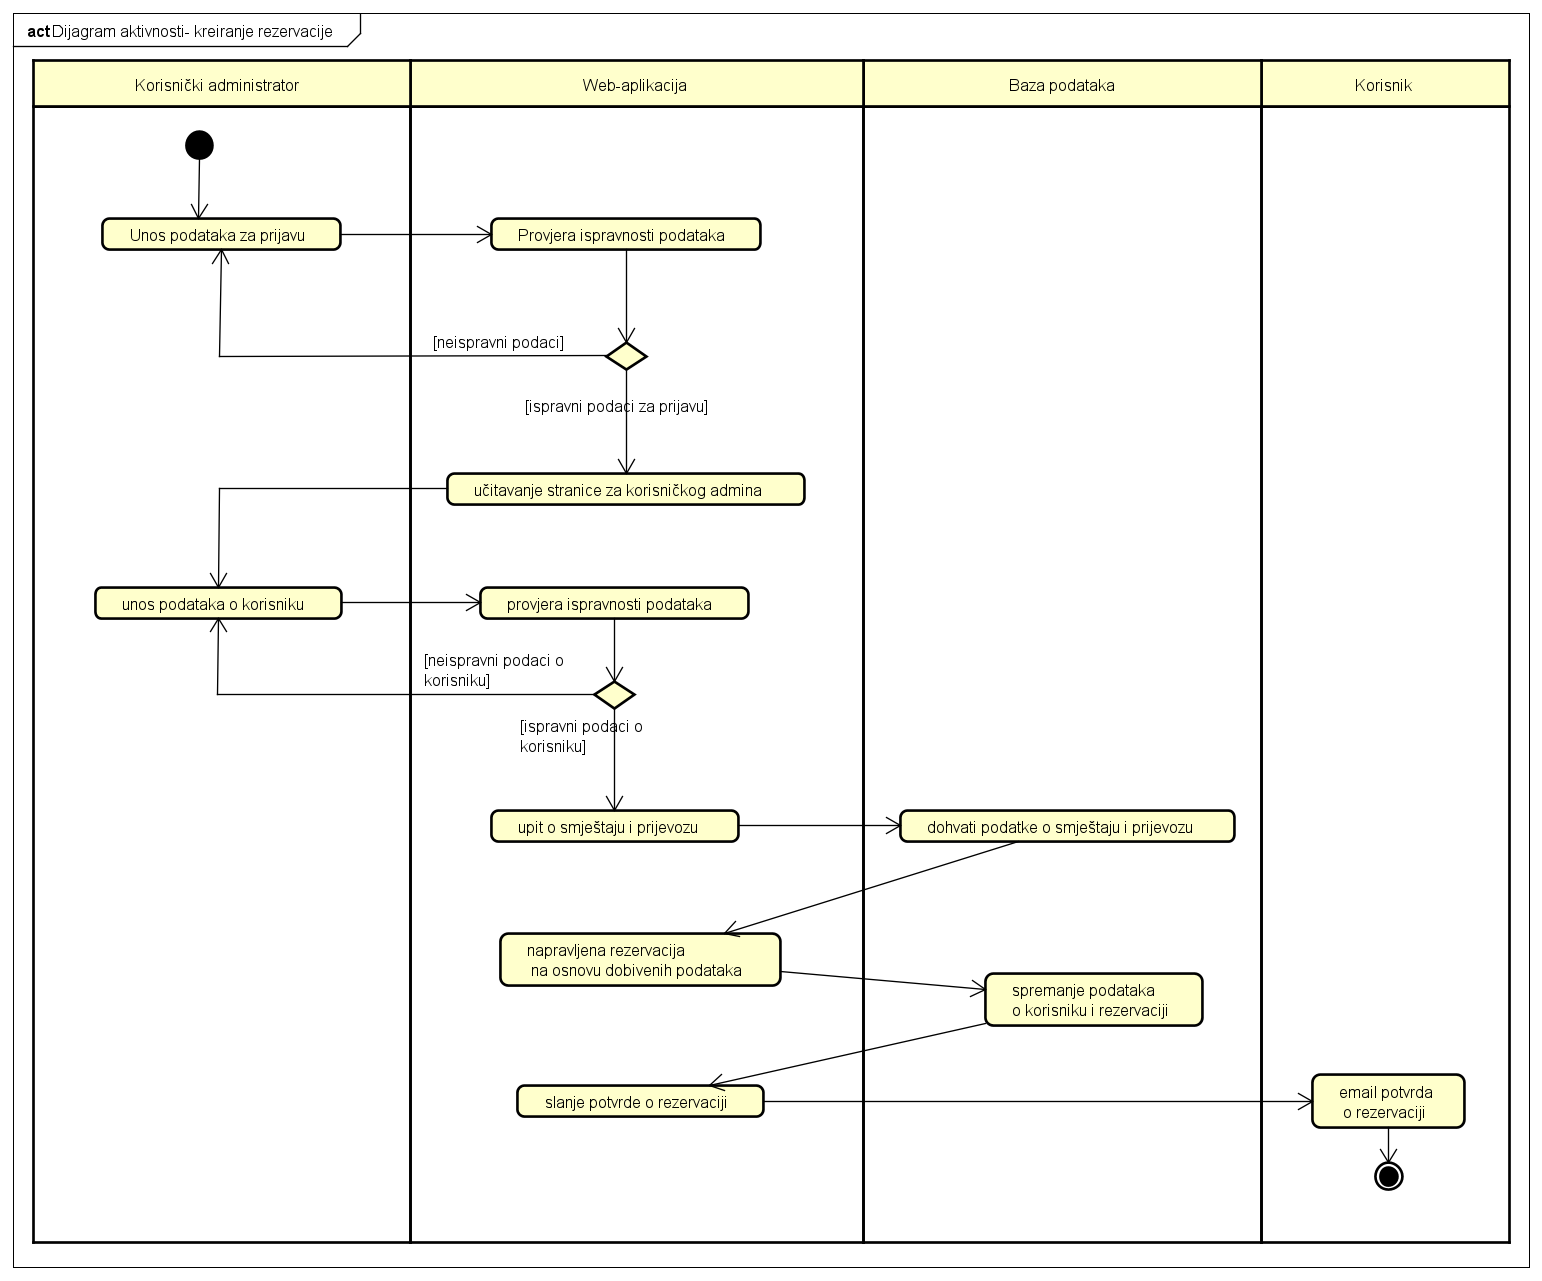
\includegraphics[width=0.9\textwidth]{dijagrami/dijagramAktivnosti.png}
			 	\caption{Dijagram aktivnosti}
			 	\label{fig:dijaramAktivnosti}
			 \end{figure}
			
			\eject
		\section{Dijagram komponenti}
		
			Na slici~\ref{fig:DijagramKomponenti} prikazan je dijagram komponenti. Za dohvaćanje HTML, CSS i JS datoteka na klijentsku stranu (\textit frontend) koristi se prvo od dva sučelja. Ovisno o potrebnom prikazu (HousingAdminView, TransportAdminView, UserAdminView, Index), Router komponenta određuje koje se HTML, CSS i JS datoteke poslužuju na prvom sučelju. Sučelju za primanje JSON podataka pristupa se putem REST API komponenti. REST API pruža podatke koji pripadaju serverskoj strani aplikacije (\textit backend). Java Persistence API omogućava dohvaćanje podataka iz baze generirajući SQL upite te upisivanje u bazu. Na serverskoj strani implementiramo kontrolere (Controllers) kako bismo prenijeli modele, pretvorene u DTO (Data Transfer Object), prema klijentskoj strani dijela aplikacije.
			 \begin{figure}[htbp]
			 	\centering
			 	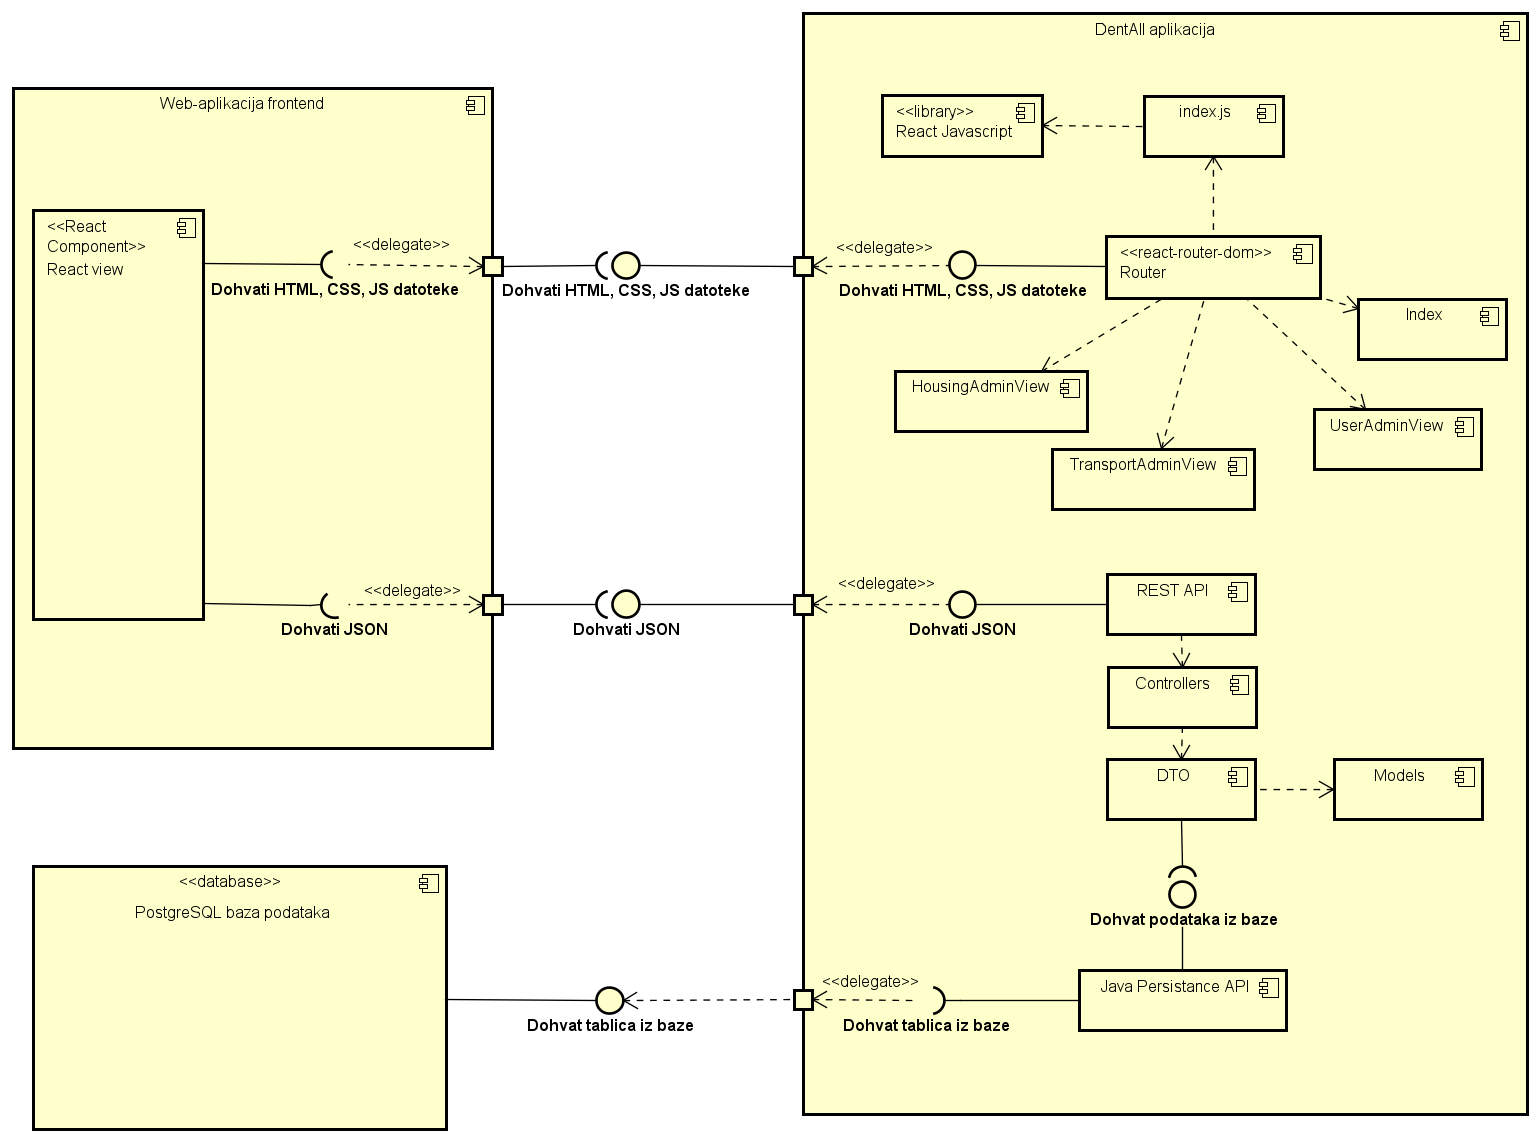
\includegraphics[width=0.9\textwidth]{dijagrami/DijagramKomponenti.png}
			 	\caption{Dijagram komponenti}
			 	\label{fig:DijagramKomponenti}
			 \end{figure}